%% LaTeX2e class for student theses
%% sections/preliminary.tex
%% 
%% Karlsruhe Institute of Technology
%% Institute for Program Structures and Data Organization
%% Chair for Software Design and Quality (SDQ)
%%
%% Dr.-Ing. Erik Burger
%% burger@kit.edu
%%
%% Version 1.1, 2014-11-21


\chapter{Fundamentals}
\label{ch:fund}

In the following chapter we want to define and explain terms and concepts used throughout this thesis as well as give an outlook to related work and the general language identification approaches.

\section{Janus Recognition Toolkit (jrtk)}
\label{sec:fund:jrtk}
The Janus Recognition Toolkit (jrtk) also known as just ``Janus'' is a general-purpose speech recognition toolkit developed in joint cooperation by both the Carnegie Mellon University Interactive Systems Lab and the Karlsruhe Institute of Technology Interactive Systems Lab~\cite{lavie1997janus}. Part of janus and the jrtk are a speech-to-speech translation system which includes Janus-SR the speech recognition component, the main part of janus used in this thesis. 

Developed to be flexible and extensible, the jrtk can be seen as a programmable shell with janus functionality being accessible through objects in the tcl/tk scripting language. It features the IBIS decoder, that uses Hidden Markov Models for acoustic modeling in general, although in this thesis we used a neural network as our speech recognizer to generate the input features required by our Language ID network.

This thesis makes extensive use of the jrtk's and tcl/tk's scripting capabilities to be able to pre-process speech audio files for further use by our experimental setup. It also uses tcl/tk scripts and it's janus API functionality in the development of our smoothing and evaluation scripts as can be seen in Ch.~\ref{ch:eval}.
\section{Neural Networks}
\label{sec:fund:NN}
Artificial Neural Networks today are used in many different fields: from image recognition/face recognition in~\cite{lawrence1997face} to Natural Language Processing in~\cite{collobert2008unified} and, as relevant to this thesis, to Speech Recognition and very successfully as in~\cite{hinton2012deep}. It has also been used in the realm of Language Identification, which will be described in Sec.~\ref{sec:fund:work}. This section will provide fundamental knowledge of how neural networks work and how to train them, to make the understanding of later chapters easier for the reader. The information in this section is based mostly on~\cite{haykin2004comprehensive}.

\subsection{General Setup}
\label{sec:fund:general}
Neural Networks are based on collections of small ''neural units``  working together in tandem. The neuron's behavior can be loosely linked to the brain's axons. Each neuron is connected with others and a neuron is ''stimulated`` by input on these connections and then decides on its own activation, or stimulation, by using a summation, or threshold, function with a certain limit to decide if the neuron ''fires`` and its own activation is propagated through the network to adjacent units. By changing weigths and activation thresholds in the network its output changes, therefore the training of artificial networks is done by adjusting the connection weights between neurons as well as the thresholds for its activation functions. 
\subsection{Artificial Neuron}
\label{sec:fund:AN}

An artificial neuron is a mathematical function that consists of four parameters that can be adjusted independently from each other:
\begin{itemize}
\item \(w_i\) the input weights for all inputs
\item \(\Sigma\) the transfer function for summation of the weighted inputs
\item \(\varphi\) the activation function that calculates the output value \(y_k\) basend on the transfer input and the threshold
\item \(\theta\) the threshold which defines when the neuron activates.
\end{itemize}

This means an artificial neuron with output \(y_k\) is the function~\ref{eq:an}. Fig.~\ref{fig:neuron} showcases this as well. Many of these neurons coupled together (via the output of a neuron on a previous layer becoming the input for one on the current layer), make an Artificial Neural Network as used in this thesis. 

\begin{equation}
y_k = \varphi(\sum_{j=0}^{m} w_{kj}x_j) - \theta_j
\label{eq:an}
\end{equation}

\begin{figure}[h!]
\label{fig:neuron}
\caption{A schematic drawing of a Neuron and it's parameters}
\centering
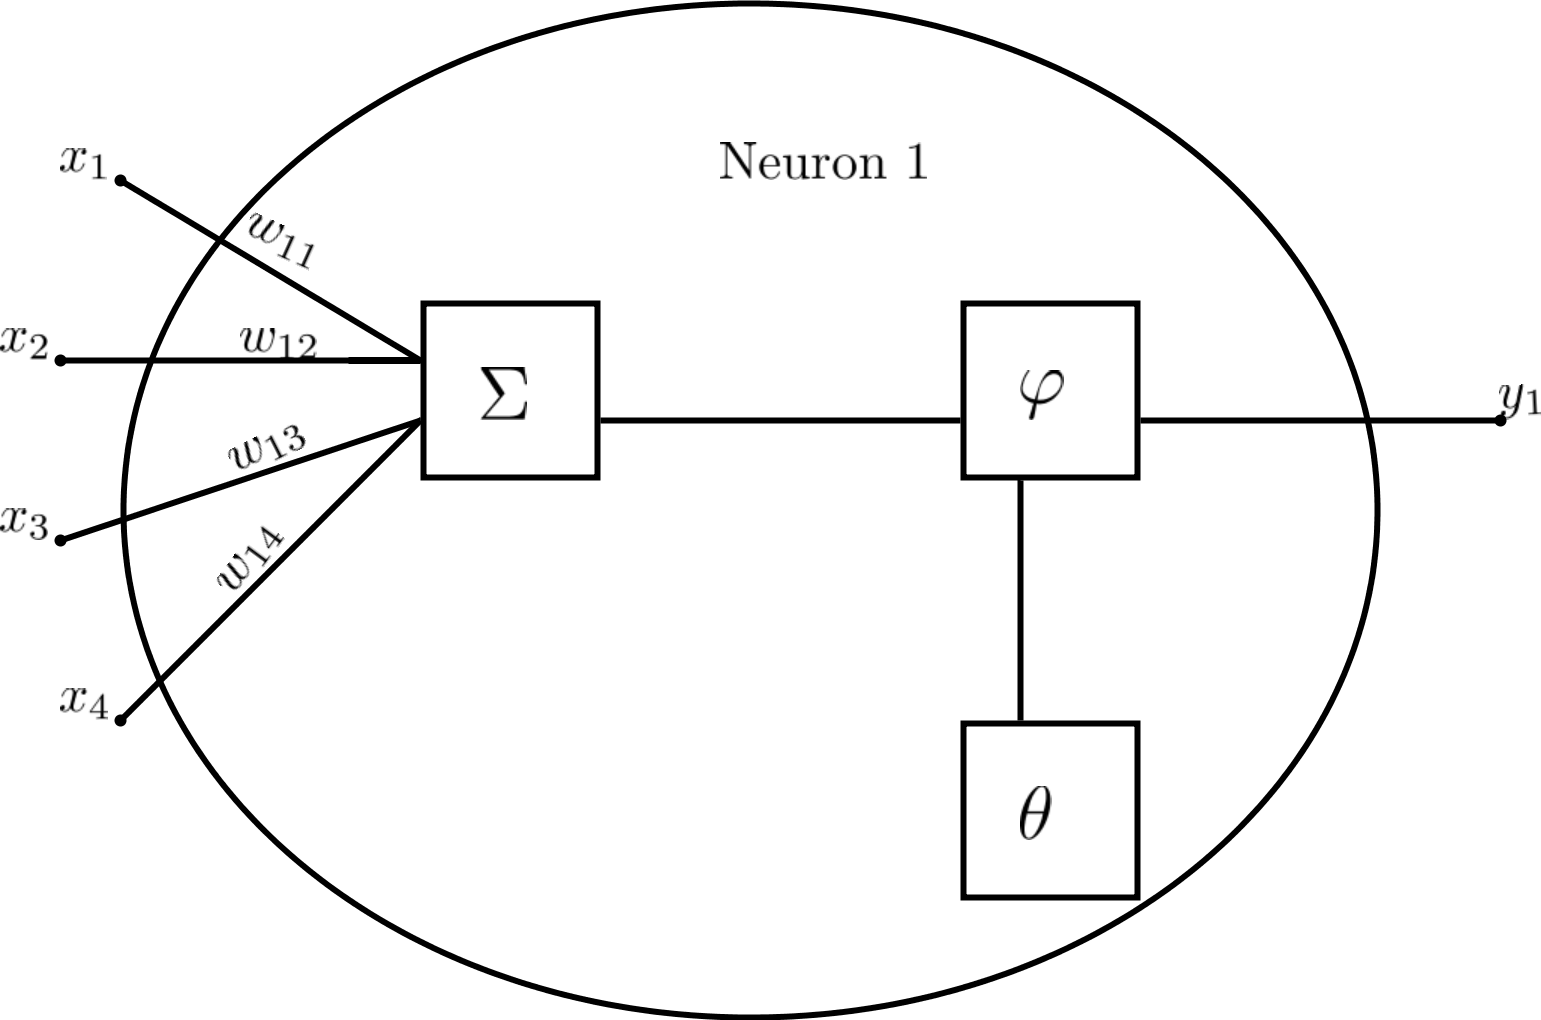
\includegraphics[width=0.7\textwidth]{images/neuron.png}
\end{figure}

\subsection{Deep Neural Networks}
\label{sec:fund:DNN}

A basic (non-deep) neural network consists of three layers: the input, a hidden layer of neurons and the output layer. Hereby, the output layer consists of as many neurons as classes that the network is trying to classify against and the one with the highest activation after entering input, is the classification output of the net.  A basicfully-connected (referring to the connections between neurons) net can be seen in Fig.~\ref{fig:net}.

Deep Neural Networks, DNNs, refer to Networks that have more than one hidden layer. In general more layers of 

\begin{figure}
\label{fig:net}
\caption{A schematic drawing of a neural network}
\centering
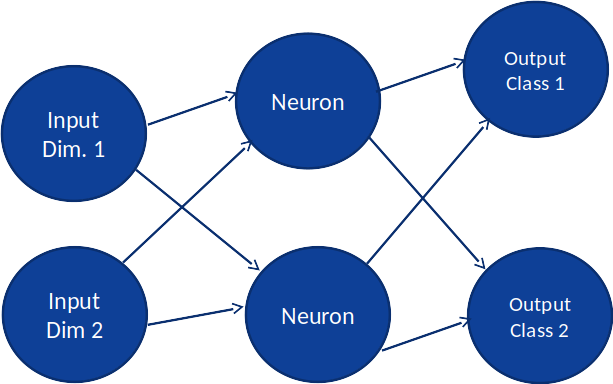
\includegraphics{images/net.png}
\end{figure}


\subsection{Training}
\label{sec:fund:Train}
Three basic approaches exist for training a neural network. This always referes to optimizing a cost function


\subsubsection{Sampling}
\label{sec:fund:Sampling}

\section{Related Work}
\label{sec:fund:work}
